\documentclass[aspectratio=169,11pt]{beamer}
% =====================================================================
%  Presentacion Tecnica del Proyecto Final - Farmacia con Consultorio Medico
%
%  Estilo MINIMALISTA MONOCROMATICO: texto NEGRO sobre fondo BLANCO.
%  Unico elemento de marca: el LOGO de Tecmilenio SOLO en la portada.
%
%  ALINEACION:
%   - Secciones = las que dicta "Presentacion del Proyecto Final.md"
%     (Exposicion oral: empresa, problematica, impacto, estrategia,
%      como ayuda la BD, beneficios, importancia de...).
%   - Contenido orientado a la RUBRICA evaluable (100 pts):
%       1) Claridad del objetivo (SMART)        -> diapositiva "Objetivo del proyecto"
%       2) Investigacion y analisis             -> problematica/impacto/estrategia fundamentados
%       3) Desarrollo y estructura              -> secuencia logica de secciones
%       4) Presentacion y comunicacion          -> diseno limpio + diagrama a pantalla completa
%
%  Compilar:  latexmk -pdf slides.tex
% =====================================================================

\usetheme{default}
\usecolortheme{dove}
\usefonttheme{professionalfonts}
\setbeamertemplate{navigation symbols}{}
\beamertemplatenavigationsymbolsempty

% --- Monocromatico: negro sobre blanco ---
\setbeamercolor{background canvas}{bg=white}
\setbeamercolor{normal text}{fg=black,bg=white}
\setbeamercolor{frametitle}{fg=black,bg=white}
\setbeamercolor{title}{fg=black}
\setbeamercolor{subtitle}{fg=black}
\setbeamercolor{author}{fg=black}
\setbeamercolor{institute}{fg=black}
\setbeamercolor{date}{fg=black}
\setbeamercolor{item}{fg=black}
\setbeamercolor{itemize item}{fg=black}
\setbeamercolor{itemize subitem}{fg=black}
\setbeamercolor{enumerate item}{fg=black}
\setbeamercolor{section in toc}{fg=black}
\setbeamercolor{caption name}{fg=black}
\setbeamercolor{block title}{fg=black,bg=white}
\setbeamercolor{block body}{fg=black,bg=white}
\setbeamertemplate{itemize items}{--}
\setbeamertemplate{enumerate items}[default]
\setbeamertemplate{sections/subsections in toc}[square]

\usepackage[utf8]{inputenc}
\usepackage[T1]{fontenc}
\usepackage[spanish]{babel}
\usepackage{graphicx}
\usepackage{tikz}

\title{Farmacia con Consultorio Médico}
\subtitle{Presentación Técnica del Proyecto Final — Base de Datos Relacional}
\author{[Tu Nombre]}
\institute{LSTI2311: Bases de Datos}
\date{\today}

\newcommand{\captura}[1]{%
  \begin{center}
  \fbox{\parbox[c][3.4cm][c]{0.86\linewidth}{\centering [Captura de pantalla: #1]}}
  \end{center}}

\begin{document}

% =====================================================================
%  PORTADA (unico lugar con el logo de Tecmilenio)
% =====================================================================
\begin{frame}[plain]
  \begin{tikzpicture}[overlay,remember picture]
    \node[anchor=north east] at ([xshift=-0.9cm,yshift=-0.7cm]current page.north east)
      {
\includegraphics[height=1.1cm]{../../../attachments/Tecmilenio Logo.png}};
  \end{tikzpicture}
  \titlepage
\end{frame}

% =====================================================================
%  AGENDA
% =====================================================================
\begin{frame}{Agenda}
  \tableofcontents
\end{frame}

% =====================================================================
%  (Exposicion oral - documento) ¿QUE EMPRESA REPRESENTAN?
% =====================================================================
\section{La empresa}
\begin{frame}{¿Qué empresa representamos?}
  \begin{itemize}
    \item Consultorio médico con farmacia asociada.
    \item Atiende consultas, emite recetas y surte medicamentos en el mismo lugar.
    \item Áreas involucradas: consultorio (médicos), farmacia (dispensación),
          compras (proveedores) y administración.
  \end{itemize}
\end{frame}

% =====================================================================
%  ¿CUAL ES SU PROBLEMATICA ACTUAL?  (rubrica: Investigacion y analisis)
% =====================================================================
\section{Problemática actual}
\begin{frame}{¿Cuál es su problemática actual?}
  \begin{itemize}
    \item Historiales clínicos en papel: se extravían y fragmentan la atención.
    \item Inventario sin control: desabasto de fármacos clave y mermas por caducidad.
    \item Recetas y ventas desvinculadas: no hay trazabilidad receta--venta.
    \item Procesos manuales: reposición tardía y errores de dispensación.
  \end{itemize}
\end{frame}

% =====================================================================
%  ¿CUAL ES SU IMPACTO?
% =====================================================================
\section{Impacto}
\begin{frame}{¿Cuál es su impacto?}
  \begin{itemize}
    \item \textbf{Clínico:} riesgo para el paciente por alergias/interacciones no detectadas.
    \item \textbf{Económico:} pérdidas por caducidad, desabasto y ventas no registradas.
    \item \textbf{Operativo:} decisiones de compra sin datos y auditorías difíciles.
    \item \textbf{Reputacional:} menor confianza del paciente en la atención.
  \end{itemize}
\end{frame}

% =====================================================================
%  OBJETIVO DEL PROYECTO (SMART)  ->  RUBRICA criterio 1: Claridad del objetivo
% =====================================================================
\section{Objetivo del proyecto}
\begin{frame}{Objetivo del proyecto (SMART)}
  \begin{block}{Objetivo}
    Implementar una base de datos relacional para el consultorio-farmacia que
    centralice historial clínico, inventario y ventas, con validaciones
    automáticas, reduciendo errores de dispensación y desabasto.
  \end{block}
  \begin{itemize}
    \item \textbf{Específico:} historial, inventario y recetas en una sola base.
    \item \textbf{Medible:} 20 tablas, 3 vistas, 3 SP y 2 triggers operativos.
    \item \textbf{Alcanzable:} MySQL + acceso desde Java (JDBC).
    \item \textbf{Relevante:} ataca las causas de riesgo clínico y pérdidas.
    \item \textbf{Temporal:} entregable al cierre del proyecto final.
  \end{itemize}
\end{frame}

% =====================================================================
%  ESTRATEGIA: causa raiz OPERATIVA antes de la tecnologia
% =====================================================================
\section{Estrategia}
\begin{frame}{Estrategia: atacar la causa raíz operativa}
  \textbf{Primero la operación, luego la tecnología.}
  \begin{itemize}
    \item Estandarizar el flujo: paciente $\rightarrow$ consulta $\rightarrow$ receta $\rightarrow$
          surtido $\rightarrow$ venta $\rightarrow$ inventario $\rightarrow$ reposición.
    \item Definir reglas de negocio: vigencia de cédula médica, control de
          alergias/interacciones, stock mínimo y caducidad.
    \item Después, llevar esas reglas a la base de datos como
          restricciones, procedimientos y triggers.
  \end{itemize}
\end{frame}

% =====================================================================
%  IMPORTANCIA DE... (documento)
% =====================================================================
\begin{frame}{¿Cuál es la importancia de...?}
  \begin{itemize}
    \item \textbf{Entender las reglas de negocio:} evita errores clínicos y define
          qué debe validar el sistema.
    \item \textbf{Mapear el flujo de información:} muestra qué datos se comparten
          entre consultorio, farmacia y compras.
    \item \textbf{Integrar operación y tecnología:} una sola fuente de verdad,
          sin islas de información.
    \item \textbf{Gestionar la ejecución de la estrategia:} vistas, SP y triggers
          garantizan que las reglas se cumplan.
  \end{itemize}
\end{frame}

% =====================================================================
%  MODELO ER a PANTALLA COMPLETA (solo)  -> Presentacion y comunicacion
% =====================================================================
\section{Modelo Entidad-Relación}
{%
\setbeamertemplate{footline}{}%
\begin{frame}[plain]
  \begin{center}
    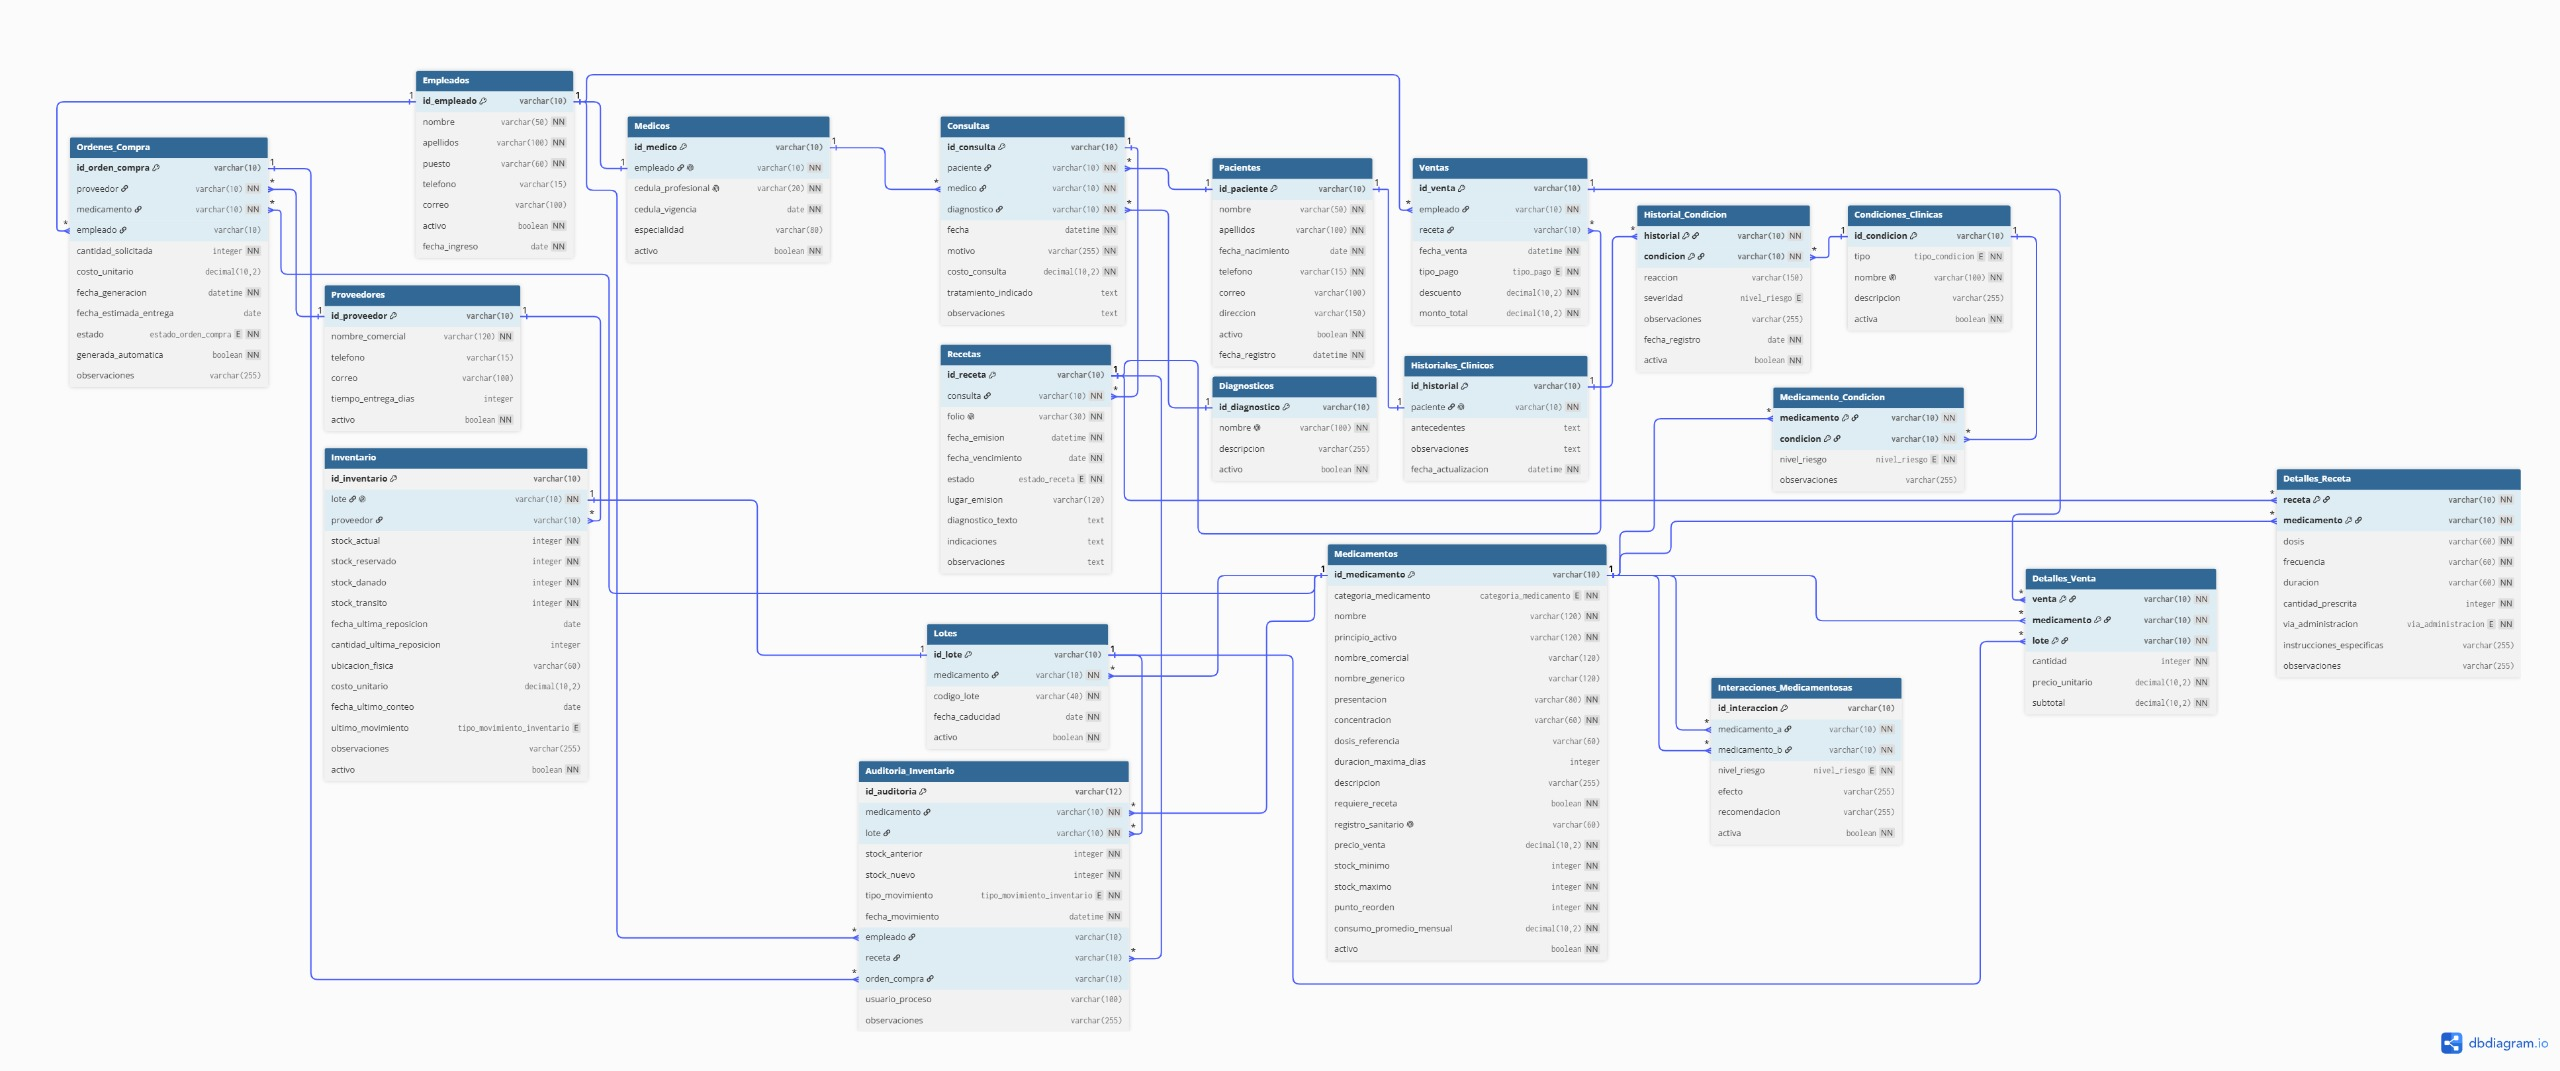
\includegraphics[width=\paperwidth,height=\paperheight,keepaspectratio]{../../../attachments/WhatsApp Image 2026-09-25 at 09.53.27.jpeg}
  \end{center}
\end{frame}
}

\begin{frame}{Modelo Entidad-Relación: estructura}
  \textbf{20 tablas} organizadas en:
  \begin{itemize}
    \item Personas: Empleados, Médicos, Pacientes.
    \item Clínico: Historiales, Condiciones, Consultas, Recetas.
    \item Farmacia: Medicamentos, Lotes, Inventario.
    \item Comercial: Ventas, Proveedores, Órdenes de Compra.
    \item Auditoría: \texttt{Auditoria\_Inventario} (LOG).
  \end{itemize}
  \vspace{0.4em}
  Claves primarias y foráneas por tabla; convención de IDs con prefijo
  (p.\,ej. \texttt{PAC-000001}). Normalización 1FN--3FN.
\end{frame}

% =====================================================================
%  ¿COMO AYUDARIA LA BD? - GESTION DE DATOS  (Vistas)
% =====================================================================
\section{¿Cómo ayuda la BD? — Gestión de datos}
\begin{frame}{¿Cómo ayuda la BD en la gestión de los datos? (Vistas)}
  \begin{itemize}
    \item \textbf{Vista 1 --- Historial clínico completo del paciente.}
      Consolida consultas, diagnósticos, recetas, dosis y alergias.
    \item \textbf{Vista 2 --- Inventario con alertas de stock mínimo.}
      Estado (suficiente/bajo/crítico/agotado), lote y caducidad más próxima.
    \item \textbf{Vista 3 --- Medicamentos más recetados y surtidos.}
      Conversión receta--venta y tendencia de consumo para decidir compras.
  \end{itemize}
  \captura{resultado de una vista en MySQL}
\end{frame}

% =====================================================================
%  ¿COMO AYUDARIA LA BD? - AUTOMATIZACION (Stored Procedures)
% =====================================================================
\section{¿Cómo ayuda la BD? — Automatización}
\begin{frame}{Automatización de procesos: Stored Procedures}
  \begin{itemize}
    \item \textbf{SP1 --- Registrar consulta y emitir receta.}
      Valida paciente activo, médico con cédula vigente y alergias;
      inserta consulta, receta y detalle.
    \item \textbf{SP2 --- Surtir receta y actualizar inventario.}
      Verifica vigencia, asigna lote no vencido, registra la venta y
      descuenta stock automáticamente.
    \item \textbf{SP3 --- Generar órdenes de reposición por stock mínimo.}
      Evalúa stock $\leq$ mínimo y crea la orden sin duplicados.
  \end{itemize}
\end{frame}

\begin{frame}{Automatización y trazabilidad: Triggers y LOG}
  \begin{itemize}
    \item \textbf{Trigger 1 --- \texttt{BEFORE INSERT} en \texttt{Detalles\_Receta}.}
      Bloquea recetas con contraindicaciones, interacciones o datos inválidos.
    \item \textbf{Trigger 2 --- \texttt{AFTER UPDATE} en \texttt{Inventario}.}
      Registra cada movimiento de stock en la tabla LOG
      \texttt{Auditoria\_Inventario} para trazabilidad total.
  \end{itemize}
  \vspace{0.3em}
  \small\textit{La automatización aplica las reglas de negocio sin intervención manual.}
\end{frame}

% =====================================================================
%  CONEXION JAVA (JDBC) - datos en uso
% =====================================================================
\section{Conexión Java (JDBC)}
\begin{frame}{Los datos en uso: conexión Java (JDBC)}
  \begin{itemize}
    \item \texttt{App.java} conecta a MySQL (instancia gestionada en Aiven, SSL).
    \item Credenciales fuera del código (variables de entorno seguras).
    \item Consulta \texttt{Pacientes} y despliega el Dataset resultante.
  \end{itemize}
  \captura{salida de la ejecución de \texttt{App.java}}
\end{frame}

% =====================================================================
%  VALIDACION (documento pide al menos 3 ejemplos de SP/Trigger)
% =====================================================================
\section{Validación}
\begin{frame}{Validación: 3 ejemplos de SP y Triggers}
  \begin{enumerate}
    \item \textbf{SP1:} receta a paciente con alergia $\Rightarrow$ el sistema la
          rechaza con mensaje de riesgo clínico.
    \item \textbf{SP2:} surtir receta vigente $\Rightarrow$ se registra la venta y
          disminuye el stock.
    \item \textbf{Trigger 2:} tras el surtido $\Rightarrow$ registro automático en
          \texttt{Auditoria\_Inventario}.
  \end{enumerate}
  \captura{ejecución de los 3 ejemplos con su resultado}
\end{frame}

% =====================================================================
%  BENEFICIOS de la nueva estrategia y solucion (documento)
% =====================================================================
\section{Beneficios}
\begin{frame}{¿Qué beneficios se obtendrán?}
  \begin{itemize}
    \item \textbf{Atención más segura:} validaciones clínicas automáticas.
    \item \textbf{Menos pérdidas:} control de inventario, caducidades y reposición.
    \item \textbf{Trazabilidad:} vínculo receta--venta y auditoría de inventario.
    \item \textbf{Mejores decisiones:} reportes de consumo para compras.
    \item \textbf{Escalabilidad:} base para un sistema de gestión completo.
  \end{itemize}
\end{frame}

% =====================================================================
%  CONCLUSION
% =====================================================================
\section{Conclusión}
\begin{frame}{Conclusión}
  \begin{itemize}
    \item El problema operativo se atacó antes de la solución tecnológica.
    \item La base de datos integra historial, inventario y ventas con reglas
          de negocio automatizadas.
    \item Resultado: atención más segura, menos pérdidas y trazabilidad total.
  \end{itemize}
\end{frame}

\begin{frame}[plain]
  \begin{center}
    \Large Gracias\\[0.4em]
    \normalsize ¿Preguntas?
  \end{center}
\end{frame}

\end{document}
